\documentclass[a4paper, 11pt]{article} % Font size (can be 10pt, 11pt or 12pt) and paper size (remove a4paper for US letter paper)
\usepackage{helvet}
\renewcommand{\familydefault}{\sfdefault}
\usepackage[protrusion=true,expansion=true]{microtype} % Better typography
\usepackage{graphicx} % Required for including pictures
\usepackage[usenames,dvipsnames]{color} % Coloring code
\usepackage{wrapfig} % Allows in-line images
\usepackage[utf8]{inputenc}
\usepackage{enumerate}
\usepackage{enumitem}

% Imágenes
\usepackage{graphicx} 

\usepackage{amsmath}
% para importar svg
%\usepackage[generate=all]{svgfig}

% sudo apt-get install texlive-lang-spanish
\usepackage[spanish]{babel} % English language/hyphenation

% Hay que pelearse con babel-spanish para el alineamiento del punto decimal

\usepackage{dcolumn}
%\newcolumntype{d}[1]{D{.}{\esperiod}{#1}}
\makeatletter

\makeatother

\usepackage{longtable}
\usepackage{tabu}
\usepackage{supertabular}

\usepackage{multicol}
%\newsavebox\ltmcbox

% Para algoritmos
\usepackage{algorithm}
\usepackage{algorithmic}
\usepackage{amsthm}
\usepackage{multirow} % para las tablas
% Para matrices
\usepackage{amsmath}

% Símbolos matemáticos
\usepackage{amssymb}
\usepackage{accents}
%\let\oldemptyset\emptyset
%\let\emptyset\varnothing

\usepackage[hidelinks]{hyperref}

\usepackage[section]{placeins} % Para gráficas en su sección.
\usepackage[T1]{fontenc} % Required for accented characters
\usepackage{tikz}
\newenvironment{allintypewriter}{\ttfamily}{\par}
\setlength{\parindent}{0pt}
\parskip=8pt
\linespread{1.05} % Change line spacing here, Palatino benefits from a slight increase by default

\makeatletter
\renewcommand\@biblabel[1]{\textbf{#1.}} % Change the square brackets for each bibliography item from '[1]' to '1.'
\renewcommand{\@listI}{\itemsep=0pt} % Reduce the space between items in the itemize and enumerate environments and the bibliography
\newcommand{\imagen}[2]{\begin{center} \includegraphics[width=90mm]{#1} \\#2 \end{center}}
\newcommand{\RFC}[1]{\href{https://www.ietf.org/rfc/rfc#1.txt}{RFC-#1}}

\renewcommand{\maketitle}{ % Customize the title - do not edit title and author name here, see the TITLE block below
	\begin{center} % Center align
		{\Huge\@title} % Increase the font size of the title
	\end{center}
	
	\vspace{20pt} % Some vertical space between the title and author name
	
	\begin{flushright} % Right align
		{\large\@author} % Author name
		\\\@date % Date
		
		\vspace{40pt} % Some vertical space between the author block and abstract
	\end{flushright}
	\renewcommand{\baselinestretch}{0.5}
	
}


\usepackage[a4paper]{geometry}
\geometry{top=2cm, bottom=2cm, left=2.25cm, right=2.25cm}






\title{\textbf{Proyecto de Prácticas}\\ % Title
\vspace{20 pt}Página Web de un grupo de investigación.
} % Subtitle

\author{\textsc{Daniel López García} % Author
\\{\textit{Universidad de Granada}}} % Institution

\date{\today} % Date

\newcounter{ndef}

\begin{document}
	\maketitle
\section{Manual de usuario.}
\section{Diseño de la base de datos.}
He realizado la simplificación de considerar un único tipo de publicación, ya que la única variación que aporta es a nivel de base de datos. En caso de querer considerar varios tipos de publicación para listar las publicaciones bastaría con tener una vista en la base de datos que unificara todos los tipos y mostrar las tuplas de esa vista. 
\medskip

A continuación se muestra un diagrama que resume la base de datos:
\begin{figure}[H]
	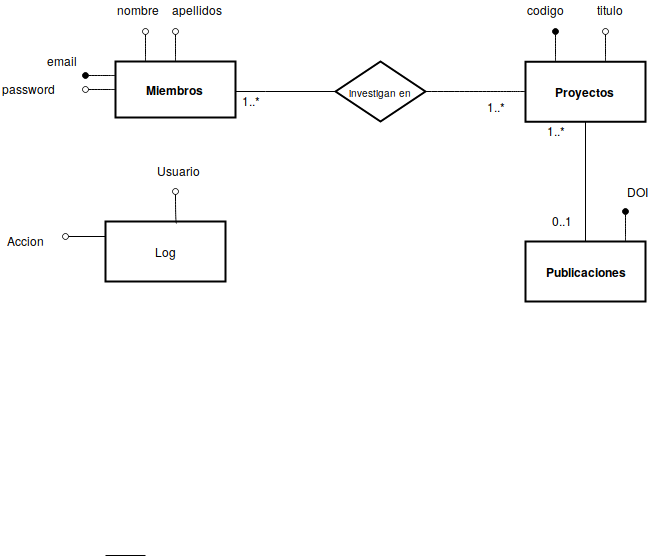
\includegraphics[scale=0.65]{./diagrama_er.png}
\end{figure}

	
\medskip
Las tablas son las siguientes:
\begin{itemize}
	\item Miembros.
	\item Proyectos.
	\item Publicaciones.
	\item Log
\end{itemize}
\section{Aspectos relevantes del desarrollo.}
\subsection{HTML y CSS.}
\subsection{PHP.}
En la carpeta \emph{\/php} se encuentran los archivos que realizan los procedimientos PHP. A continuacion se detallan dichos archivos:
\begin{itemize}
	\item borrar.php
	\item editar.php. Muestra los formularios de edición.
	\item backup.php. Realiza un backup de la base de datos y guarda las sentencias SQL en un archivo cuyo nombre se forma con la fecha y hora actuales. 
	\item restaurarBD.php. Lee y ejecuta las sentencias SQL del último archivo de backup para restaurar la base de datos. 
	\item db.php. Contiene las funciones que realizan llamadas a la base de datos.
	\item nuevoMiembro.php, nuevoProyecto.php, nuevaPublicacion.php. Obtienen los datos de los formularios correspondientes y realizan una llamada a la base de datos.
	\item editarMiembro.php,editarProyecto.php,editarPublicacion.php. Obtienen los datos de los formularios correspondientes y realizan una llamada a la base de datos.
	\item borrarMiembro.php,borrarPublicacion.php, borrarProyecto.php
    \item listMiembros.php,listProyectos.php,listPublicaciones.php, listLog.php. Obtienen los datos almacenados en la base de datos y los listan añadiendo cuando es posible los botones que posibilitan la edición y el borrado.
    \item login.php,logout.php. Gestionan el login en el sistema mediante el uso de sesiones.
	
\end{itemize}
\end{document}